\chapter{Esercizi}
\label{chap:esercizi}

\section{Esercizio 1}
\label{sec:esercizio1}

\begin{eqnarray*}
  \begin{cases}
    x+y+z=1\\
    2x-y-z=0
  \end{cases} & A/b=
                \left(\begin{array}{ccc|l}
                  1&1&1 & 1 \\
                  2 & -1 & -1 &0
                \end{array}\right)
\end{eqnarray*}

\subsection{Riduzione a gradini:}
\label{sec:riduzioneagradini}

\subsubsection{$1^o$ soluzione}
\label{sec:soluzione1}

\begin{eqnarray*}
 2\left(
  \begin{array}{ccc|l}
    1&1&1 &1\\
    2 & -1 & -1 & 0
  \end{array}\right) R_2\to R_2-2R_1 \left(
  \begin{array}{ccc|l}
    1&1&1&1\\
    0 & -3 & -3&-2
  \end{array} \right)
\end{eqnarray*}
\begin{eqnarray*}
  \left(
  \begin{array}{ccc|l}
    1&1&1&1\\
    0 & -3 & -3&-2
  \end{array} \right) &
                        \begin{matrix}
                          rg(A/b)=2\\
                          \infty^{n-2g(A)} \to \infty^{3-2} = \infty^1
                        \end{matrix}
\end{eqnarray*}

\subsubsection{$2^o$ soluzione}
\label{sec:soluzione2}

\begin{eqnarray*}
  \left(
  \begin{array}{ccc|l}
    1&1&1&1\\
    0 & -3 & -3&-2
  \end{array} \right)&\to&
                           \begin{cases}
                             x+y+z=1\\
                             -3y-3z=-2
                           \end{cases}
\end{eqnarray*}
\begin{eqnarray*}
  =
  \begin{cases}
    x+y+z=1\\
    y=\frac{2}{3}-z
  \end{cases}&\to&
  \begin{cases}
    x=1\left(\frac{2}{3}-z\right)-z\\
    y=\frac{2}{3}-z
  \end{cases}=
                   \begin{cases}
                     x=\frac{1}{3}\\
                     y=\frac{2}{3}-z
                   \end{cases}\to z=t
\end{eqnarray*}
A questo punto abbiamo $V$
\begin{eqnarray*}
  V=\left(\frac{1}{2},\frac{2}{3}-t,t\right) & \forall t \in \mathds{K}
\end{eqnarray*}
\begin{eqnarray*}
  \begin{cases}
    x=\frac{1}{3}\\
    y=\frac{2}{3}-t\\
    z=t
  \end{cases} & \to &
                      \begin{matrix}
                        \text{parametriche della retta} 
                      \end{matrix}
\end{eqnarray*}
\begin{eqnarray*}
  \begin{matrix}
    n_1(1,1,1)\\
    n_2(2,-3,-3)
  \end{matrix}& n_1\wedge n_2=(0,3,-3)
\end{eqnarray*}
\clearpage
\section{Esercizio 2}
\label{sec:esercizio2}

\begin{eqnarray*}
  \begin{cases}
    x+y+2z=5
  \end{cases}
\end{eqnarray*}
La matrice risulta essere già ridotta a gradini, quindi la matrice composta da una sola riga
\begin{equation*}
  (\begin{array}{ccc|c}
    1&1&2&5
  \end{array})
\end{equation*}
\begin{eqnarray*}
  y=t, & z=s, & x=5-t-2s
\end{eqnarray*}
\begin{equation*}
  \begin{cases}
    x=5-t-2s\\
    y=t\\
    z=s
  \end{cases}
\end{equation*}

\section{Esercizio 3}
\label{sec:esercizio3}
\begin{equation*}
  \vec{OP}_1,\vec{OP}_2,\vec{OP}_3
\end{equation*}
Partendo da questa base possiamo andare a svilupparlo nel seguente modo:
\begin{eqnarray*}
  \vec{OP}_1+\vec{OP}_2-\vec{OP}_3=v_1\\
  \vec{OP}_2+\vec{OP}_3=v_2\\
  \vec{OP}_1-\vec{OP}_2=v_3
\end{eqnarray*}
Ad esempio,
  \begin{figure}[ht]
    \centering
    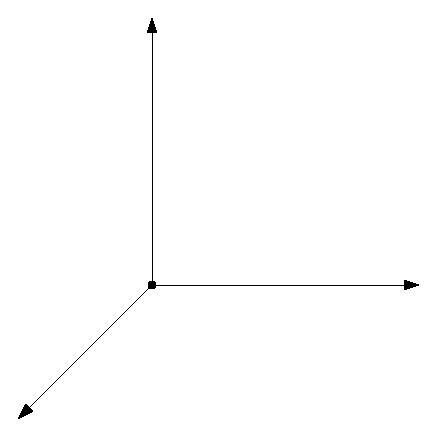
\includegraphics[width=3cm]{img/finiti/es/es1.eps}
  \end{figure}\\
$v_1,v_2,v_3$ sono ancora una base?
\begin{eqnarray*}
  \begin{array}{c}
    \vec{OP}_1+\vec{OP}_2-\vec{OP}_3\equiv (1,1,-1)\\
    \vec{OP}_1+\vec{OP}_3\equiv (0,1,2)\\
    \vec{OP}_1-\vec{OP}_2\equiv (1,-1,0)
  \end{array}&
  \begin{array}{c}
    \text{Linearmente}\\
    \text{indipendenti}
  \end{array}
\end{eqnarray*}
\begin{equation*}
  A=
  \begin{pmatrix}
    1 & 1 &-1\\
    0 & 1 & 2\\
    1 & -1 & 0
  \end{pmatrix} R_3\to R_3-R_1
  \begin{pmatrix}
    1 & 1 &-1\\
    0 & 0 & 2\\
    0 & -2 & 1
  \end{pmatrix}
\end{equation*}
\begin{equation*}
  R_3\to R_3+2R_2
  \begin{pmatrix}
    1 & 1 & -1\\
    0 & 1 & 2\\
    0 & 0 & 5
  \end{pmatrix} \text{ } rg(A)=3
\end{equation*}
\begin{eqnarray*}
  \begin{cases}
    x_1+x_2+x_3+x_4=3\\
    2x_1+x_2+x_3-x_4=5
  \end{cases} & \text{Sistema non omogeneo}\\
  \begin{cases}
     x_1+x_2+x_3+x_4=0\\
    2x_1+x_2+x_3-x_4=0   
  \end{cases} & \text{Sistema omogeneo}
\end{eqnarray*}
\clearpage
\subsection{Sistema omogeneo}
\label{sec:sistemaomogeneo}

\begin{equation*}
   \begin{cases}
     x_1+x_2+x_3+x_4=0\\
    2x_1+x_2+x_3-x_4=0   
  \end{cases}  
\end{equation*}
\begin{equation*}
  -2
  \begin{pmatrix}
    1 & 1 & 1 &1\\
    2 & 1 & 1 & -1
  \end{pmatrix} R_2\to R_2-2R_1
  \begin{pmatrix}
    1 & 1 & 1 & 1\\
    0 & -1 & -1 & -3
  \end{pmatrix}
\end{equation*}
\begin{equation*}
   \begin{pmatrix}
    1 & 1 & 1 & 1\\
    0 & -1 & -1 & -3
  \end{pmatrix}
  \begin{array}{l}
    rg (A)=2\\
    \dim(V)=4
  \end{array}
\end{equation*}
\begin{eqnarray*}
  \infty^{4-2} \text{ soluzioni }\to \infty^2 \text{ soluzioni}
\end{eqnarray*}
\begin{eqnarray*}
  \begin{pmatrix}
    1 & 1 & 1 & 1\\
    0 & -1 & -1 & -3
  \end{pmatrix}\to
  \begin{cases}
    x+y+z+w=0\\
    -y-z-3w=0
  \end{cases}\to 
  \begin{cases}
    x+y+z+w=0\\
    -y=z+3w
  \end{cases}\\
  \to \begin{cases}
    x+y+z+w=0\\
    y=-z-3w
  \end{cases}
\end{eqnarray*}
$z=t$, $w=s$
\begin{equation*}
  \begin{cases}
    x+y+t+s=0\\
    y=-t-3s
  \end{cases}\to
  \begin{cases}
    x=2s\\
    y=-t-3s
  \end{cases}
\end{equation*}
\begin{equation*}
  \text{Soluzione} \to (2s,-t-3s,t,s) \to \text{Sottospazio vettoriale di } \abs{\abs{R^4}} \to (2s,-3s,0,s)+(0,-t,t,0)
\end{equation*}
\begin{equation*}
  \boxed{s(2,-3,0,1)+t(0,-1,1,0)}\to \text{ Soluzione generale}
\end{equation*}
\begin{equation*}
  <(2,-3,0,1)(0,-1,1,0)> \text{base del sottospazio vettoriale generato}
\end{equation*}
\subsection{Sistema disomogeneo}
\label{sec:sistemadisomogeneo}

\begin{equation*}
   \begin{cases}
     x_1+x_2+x_3+x_4=3\\
    2x_1+x_2+x_3-x_4=5   
  \end{cases}  
\end{equation*}
\begin{eqnarray*}
  \left(
  \begin{array}{cccc|c}
    1&1&1&1&3\\
    2&1&1&-1&5
  \end{array}
  \right)R_2\to R_2-2R_1
  \left(
  \begin{array}{cccc|c}
    1&1&1&1&3\\
    0&1&-1&-3&-1
  \end{array}
  \right)
\end{eqnarray*}
\begin{eqnarray*}
  \begin{cases}
    x+y+z+w=3\\
    -y-z-3w=-1
  \end{cases}\to
  \begin{cases}
    x+y+z+w=3\\
    y+z+3w=1
  \end{cases}
\end{eqnarray*}
$z=t$, $w=s$
\begin{eqnarray*}
  \begin{cases}
    x=3-1+\not{t}+3s-\not{t}-s\\
    y=1-t-3s
  \end{cases}
\end{eqnarray*}
\begin{equation*}
  \begin{cases}
    x=2+2s\\
    y=1-t-3s   
  \end{cases}
\end{equation*}
\begin{eqnarray*}
  \begin{cases}
    x=2+2s\\
    y=1-t-3s\\
    z=t\\
    w=s
  \end{cases}\\
  \text{Soluzione } \to (2+2s,1-t-3s,t,s)\\
  (2,1,0,0)+(2s,-3s,0,s)+(0,-t,t,0)\\
  \boxed{(2,1,0,0)+s(2s,-3s,0,s)+t(0,-t,t,0)} \to w=\text{sottospazio vettoriale}\\
  \boxed{v+w}\to \text{sottospazio affine}
\end{eqnarray*}
\begin{figure}[ht]
    \centering
    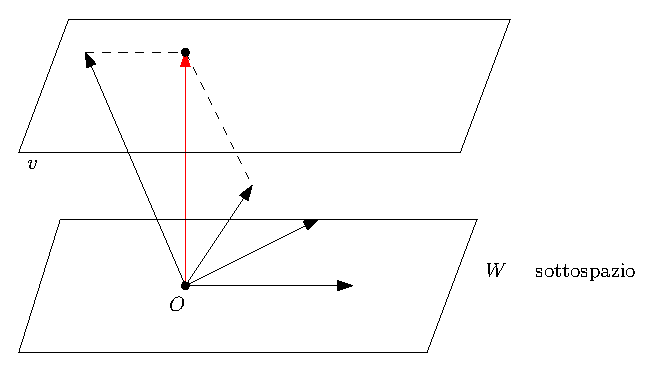
\includegraphics[width=7cm]{img/finiti/es/es2.eps}
\end{figure}

\section{Il Determinante}
\label{sec:ildeterminante}

A matrice con $
\begin{array}{|c|c}
  n & \text{righe}\\
  n & \text{colonne}
\end{array}
$\footnote{matrice quadrata $n\cdot n$}
\begin{eqnarray*}
 \begin{array}{ccc}
  M_{m,n}(\mathds{K})&\to&
                           \begin{array}{l}
                             \text{Insieme delle matrici}\\
                             \text{con $m$ riche e $n$ colonne e}\\
                             \text{a entrate $w\mathds{K}$}
                           \end{array}
 \end{array}\\
  \text{es: }
  \begin{pmatrix}
    1 & 2 & 3 \\
    4 & 5 & 6
  \end{pmatrix}\to M_{2,3}(\mathds{R})\\
  M_{n},n(\mathds{R})\\
  n(\mathds{R})\to \text{solo se quadrata}\\
  M_{n}\to \text{matrici quadrate di ordine } n\\
  \boxed{A\in M_n(\mathds{K})\Rightarrow \det(A)\in \mathds{K}}\\
  A \text{ ha rango } n \text{ (massimo) quando }\det(A)\neq 0
\end{eqnarray*}
\begin{equation*}
  \begin{pmatrix}
    a_{11} & a_{12} &\dots & a_{1n}\\
    a_{21} & a_{22} &\dots & a_{2n}\\
    \dots & &\vdots\\
    a_{n1} & a_{n2} &\dots & a_{nn} 
  \end{pmatrix}
  \begin{array}{c}
    \text{Generica}\\
    \text{matrice}\\
    \text{quadrata}
  \end{array}
\end{equation*}
\begin{equation*}
  \det(A)= \sum_{P\in S_n}\xi(P) a_1(P_1) a_2(P_2)\dots a_n (P_n)
\end{equation*}
\begin{equation*}
  \begin{pmatrix}
    a_{11} & a_{12}\\
    a_{21} & a_{22}
  \end{pmatrix}=A
\end{equation*}
\begin{equation*}
  \det(A)=(a_{11}\cdot a_{22})-(a_{12}\cdot a_{21})
\end{equation*}
Quindi prendendo andando a sostituire le variabili con i numeri esce questo
risultato
\begin{equation*}
  \begin{pmatrix}
    1 & 2 \\
    3 & 4
  \end{pmatrix}=(1 \cdot 4)- (2 \cdot 3)= 4 - 6= -2
\end{equation*}
Altro esempio,
\begin{equation*}
  \det
  \begin{pmatrix}
    1 & 2\\
    4 & 10
  \end{pmatrix}= (1* 10)-(2 * 4)= 10 - 10= 0
\end{equation*}
In questo caso vale il teorema di Laplace.
\begin{equation*}
  \det
  \begin{pmatrix}
    a_{11} & a_{12} & a_{13}\\ 
    a_{21} & a_{22} & a_{23}\\
    a_{31} & a_{32} & a_{33}
  \end{pmatrix}
  \begin{pmatrix}
    a_{11} & a_{12} & a_{13}\\ 
    a_{21} & a_{22} & a_{23}\\
    a_{31} & a_{32} & a_{33}
  \end{pmatrix}
\end{equation*}
\begin{equation*}
  a_{11}a_{22}a_{33}+a_{12}a_{23}a_{31}+a_{13}a_{21}a_{32}-\underbrace{(a_{11}a_{22}a_{33}+a_{12}a_{23}a_{31}+a_{13}a_{21}a_{32})}_{\text{Sarrus}}
\end{equation*}
\begin{equation*}
  A\in M_n(\mathds{K})\to
  \begin{array}{c}
    \text{Il determinante ha}\\
    \underbrace{n!}_{Fattoriale} \text{ addendi}
  \end{array}
\end{equation*}

\section{Formula di laplace}
\label{sec:esflaplace}

\begin{equation*}
  \begin{pmatrix}
    a_{11} & a_{12} & a_{13}\\
    a_{21} & a_{22} & a_{23}\\
    a_{31} & a_{32} & a_{33}
  \end{pmatrix}
  \begin{array}{c}
    \text{Il cofattore di } a_{23}\\
    C_{23} = \det
    \begin{pmatrix}
      a_{11} & a_{12}\\
      a_{31} & a_{32}
    \end{pmatrix}
  \end{array}
\end{equation*}
\begin{equation*}
  \begin{pmatrix}
    {\color{blue}+} & {\color{red}-} &  {\color{blue}+}\\
    {\color{red}-} &{\color{blue}+}& {\color{red}-}\\
    {\color{blue}+} & {\color{red}-} &  {\color{blue}+}
  \end{pmatrix}
\end{equation*}
Segno dei cofattori

\section{Esercizio 4}
\label{sec:esercizio4}
Prendiamo una matrice
\begin{equation*}
  \begin{pmatrix}
    
  \end{pmatrix}
\end{equation*}
